\hypertarget{near-optimal-abstractions}{%
\section{Near optimal abstractions}\label{near-optimal-abstractions}}


We are working with MDPs \((S, A, \tau, r)\), therefore we have a state
space, \(S\), an action space, \(A\), a transition function
\(P: S\times A \times S \to [0, 1]\) and a reward function
\(r: S\times A \to \mathbb R\).

Let's say we have an abstraction, (a road is a road, no real different
between them), a natural thing we want to know about the abstraction is:
is it possible for me to act optimally using this abstraction, if not,
what's the damage (in this case, of driving 100kph on every road,
because they are all prety much the same\ldots{})? Or, in other words,
which policies are approximately representable within this abstracted
MDP.

An abstract MDP is defined as;

???

The metric we are optimising is the representation error of the optimal
policy. Given an abstraction, we want to know how well the abstraction
can represent the optimal policy.

\[
\forall_{s\in S_G, a\in A_G} \mid Q_G^{\pi^* }(s, a) - Q_G^{\pi_{GA}^* }(s, a) \mid \le 2 \epsilon \eta_f
\]

We could impose properties on a state abstraction using something like
the following;


\begin{align}
\forall_{s_1, s_2 \in S} \mid f(s_1) - f(s_2)\mid \le \epsilon &\implies \phi (s_1) = \phi(s_2)\\
\forall_{\cdot} \mid f(\cdot) - f(\cdot)\mid \le \epsilon &\implies g_1(\cdot) = g_2(\cdot)\\
\end{align}


In other words, if there exists an approximate similarity, according to
\(f\), then build it into our abstraction.

\begin{itemize}
\tightlist
\item
  \textbf{Q:} How should we construct our abstraction?
\item
  \textbf{Q:} What properties should it have to achieve `good'
  performance?
\end{itemize}

Using the above method of imposing properties on an abstraction, what
should we pick as \(f\)?

\begin{enumerate}
\def\labelenumi{\arabic{enumi}.}
\tightlist
\item
  The policy function:
  \(\forall_{\cdot_a, \cdot_b \in D} \mid \pi(\cdot_a) - \pi(\cdot_b) \mid \le \epsilon\)
  is approximately the same.
\item
  The transition function:
  \(\forall_{\cdot_a, \cdot_b \in D} \mid \tau(\cdot_a) - \tau(\cdot_b)\mid \le \epsilon\)
  is approximately the same.
\item
  The reward function:
  \(\forall_{\cdot_a, \cdot_b \in D} \mid r(\cdot_a) - r(\cdot_b) \mid \le \epsilon\)
  is approximately the same.
\end{enumerate}

Also,

\begin{enumerate}
\def\labelenumi{\arabic{enumi}.}
\setcounter{enumi}{3}
\tightlist
\item
  The policy trajectory:
  \(\forall_{\cdot_a, \cdot_b \in D} \mid \sum_{t=0}^T \parallel \pi(\cdot_a) - \pi(\cdot_b)\parallel_1 \mid \le \epsilon\)
  is approximately the same.
\item
  The transition trajectory:
  \(\forall_{\cdot_a, \cdot_b \in D} \mid \sum_{t=0}^T\parallel \tau(\cdot_{a_t}) - \tau(\cdot_{b_t})\parallel_1\mid \le \epsilon\)
  is approximately the same.
\item
  The reward trajectory:
  \(\forall_{\cdot_a, \cdot_b \in D} \mid \sum_{t=0}^T \parallel r(\cdot_{a_t}) - r(\cdot_{b_t})\parallel_1 \mid \le \epsilon\)
  is approximately the same.
\end{enumerate}

GVFs

\begin{enumerate}
\def\labelenumi{\arabic{enumi}.}
\setcounter{enumi}{6}
\tightlist
\item
  The discounted future policy:
  \(\forall_{\cdot_a, \cdot_b \in D} \mid \Pi(\cdot_a) - \Pi(\cdot_b)\mid \le \epsilon\)
  is approximately the same.
\item
  The discounted future transition:
  \(\forall_{\cdot_a, \cdot_b \in D} \mid \Upsilon(\cdot_a) - \Upsilon (\cdot_b)\mid \le \epsilon\)
  is approximately the same.
\item
  The discounted future reward:
  \(\forall_{\cdot_a, \cdot_b \in D} \mid Q(\cdot_a) - Q(\cdot_b)\mid \le \epsilon\)
  is approximately the same.
\end{enumerate}

\textbf{Q:} Which is best?

\begin{quote}
\textbf{Claim 1:} 9.(the value fn) will yield the most compression,
while performing well. But, it is a task specific representation, thus
it will not transfer / generalise well.
\end{quote}

\hypertarget{other-types-of-abstraction}{%
\paragraph{Other types of
abstraction}\label{other-types-of-abstraction}}

We constructed the state abstraction by altering what the policy and
value function were allowed to see. Rather than observing the original
state space, we gave them access to an abstracted state space.

There are other ways to alter what the policy and value function sees.


\begin{align}
\phi: S \to X&: \quad \pi(s) \to \pi(\phi(s)) \quad Q(s, a) \to Q(\phi(s), a) \tag{State abstraction} \\
\psi: A\to Y&: \quad \pi(s) \to \psi^{-1}(\pi(s)) \quad Q(s, a) \to Q(s, \psi(a)) \tag{Action abstraction} \\
\phi, \psi&: \quad \pi(s) \to \psi^{-1}(\pi(\phi(s))) \quad Q(s, a) \to Q(\phi(s), \psi(a)) \tag{State and action abstraction} \\
\varphi: S \times A \to Z&: \quad \pi(s)\to \mathop{\text{argmax}}_a V(\varphi(s, a)) \quad\quad Q(s, a) \to V(\varphi(s, a)) \tag{State-action abstraction} \\
\end{align}


\begin{quote}
\textbf{Claim 2:} The state-action abstraction is the most powerful
because it allows the compression of the most symmetries. (want to
prove!)
\end{quote}

(relationship to
\href{http://www.gatsby.ucl.ac.uk/~dayan/papers/d93b.pdf}{Successor
features}!?)

State abstraction groups together states that are similar. For example,
sprinting 100m is equivalent regardless of which track lane you are in.

Action abstraction groups together actions that are similar. For
example, X and Y both yeild the state change in state, \textgreater{}
Approximation perspective: we have a set of options and we want to use
them to approximate the optimal policy. A good set of options can
efficiently achieve an accurate approximation.

\hypertarget{motivating-example-for-state-and-action-abstraction}{%
\subsubsection{Motivating example for state and action abstraction:
???}\label{motivating-example-for-state-and-action-abstraction}}

Might want to transfer. But some envs share state space, some share
action space. Want to

\begin{itemize}
\tightlist
\item
  Might be teleported to a new environment? (new state space, same
  action space)
\item
  Might have to drive a new vehicle (same state space, new action space)
\end{itemize}

\hypertarget{motivating-example-for-state-action-abstraction-symmetric-maze}{%
\subsubsection{Motivating example for state-action abstraction:
Symmetric
maze}\label{motivating-example-for-state-action-abstraction-symmetric-maze}}

\emph{(Some intuition behind claim 2.)}

Imagine you are in a mirror symmetric maze. It should not matter to you
which side of mirror you are on.

\begin{figure}
\centering
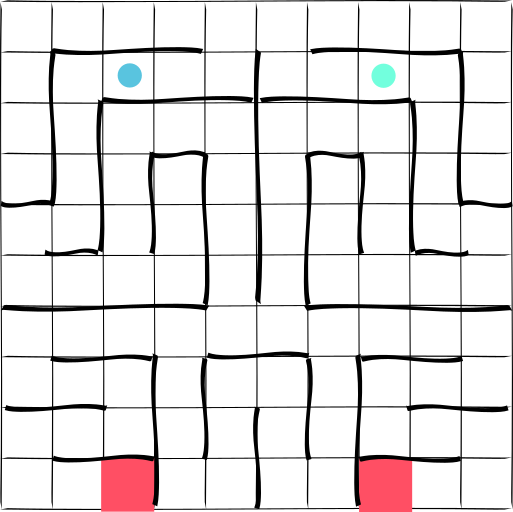
\includegraphics[width=0.5\textwidth,height=0.5\textheight]{../../pictures/drawings/maze.png}
\caption{maze.png}
\end{figure}

This reduces the state-action space by half!
\(\frac{1}{2}\mid S \mid \times \mid A \mid\). Note: just using state
abstraction it is not possible to achieve this reduction. Mirrored
states are not equivalent as the actions are inverted.

While other learners can still solve this problem. They miss out on
efficiency gains by abstracting first.

\hypertarget{related-work}{%
\subsubsection{Related work}\label{related-work}}

Other approaches to abstraction for RL focus on \ldots{}?

Near Optimal Behavior via Approximate State Abstraction \cite{Abel2017}
A Geometric Perspective on Optimal Representations for Reinforcement Learning \cite{Bellemare2019b}
successor representation

\hypertarget{discussion}{%
\subsection{Discussion}\label{discussion}}

But can we guarantee that these abstractions do not make it harder to
find the optimal policy? Is that even possible?

\begin{center}\rule{0.5\linewidth}{\linethickness}\end{center}

Want a general way (a function) to take an abstraction of an MDP
(defined by certain propreties) and return the difference between its
optimal policy and the true optimal policy. Want automated computational
complexity to solve this! Actually, we are not considering computational
complexity here only approximation error. For that can we just use
automatic differentiation!? Want a way to get bounds for all of these
combinations!

\begin{center}\rule{0.5\linewidth}{\linethickness}\end{center}

How do we know one policy is better than another? How do we know a
policy is optimal?

\[
\forall \pi\;\; V^{\pi^* } \ge V^{\pi} \\
\]

But, this definition of optimality implicitly assumes a uniform
distribution over states. This is unlikely. Rather, the distribution is
determined by the policy.

\[
\mathop{{\mathbb E}}_{s\sim D_{\pi}} \big[ V^{\pi^* } \big] \ge \mathop{{\mathbb E}}_{s\sim D_{\pi}} \big[ V^{\pi} \big] \\
D_{\pi}(s) = P(s | \pi) = \sum_{\text{all } \tau \text{ with } s_t = s} P(\tau | \pi)
\]

Now. How different is this?

I can imagine some degenerate solutions now being possible? Because we
can control the distribution we are being evaluated on. We could pick a
policy that oscillates between two states, never leaving the cycle.
Therefore it would have \(p(s_1) = p(s_2) = 0.5\) and
\(p(s_{i \neq 1,2}) = 0\).

That doesn't seem so bad?
